%% derived from https://tex.stackexchange.com/questions/357538/graph-of-a-parabola-on-pgfplots
%% Thanks to Stefan Pinnow
%%     https://tex.stackexchange.com/users/95441/stefan-pinnow

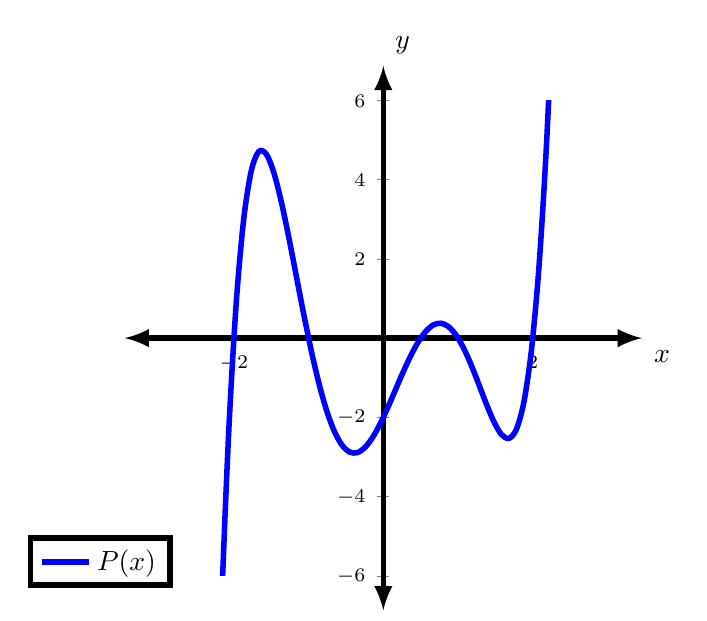
\begin{tikzpicture}
  \begin{axis}[
      samples=70,
      smooth,
      line width=2pt,
      domain=-4:3,
      legend pos=south west,
      legend style={
        anchor=east
      },
      width=0.6\textwidth,
      height=3in,
      axis lines=middle,
      xmin=-3,
      xmax=3,
      ymin=-6,
      ymax=6,
        scaled ticks=false,
        ticklabel style={font=\scriptsize},
        xlabel=$x$,
        ylabel=$y$,
        axis line style={
          latex-latex,
          shorten >=-12.5pt,
          shorten <=-12.5pt,
        },
        xlabel style={at={(ticklabel* cs:1)}, xshift=12.5pt, anchor=north west},
        ylabel style={at={(ticklabel* cs:1)}, yshift=12.5pt, anchor=south west},
    ]
    
    \addplot[color=blue] {x^5 - 0.5 * x^4 - 5* x^3 + 2.5 * x^2 + 4* x - 2};  
    \addlegendentry{\(P(x)\)}
  \end{axis}
\end{tikzpicture}
%
